%!TEX root = ../template.tex
\chapter{Refractor Telescope Design}
\label{ap:telescope_design}

\begin{figure}[htpb]
    \centering
    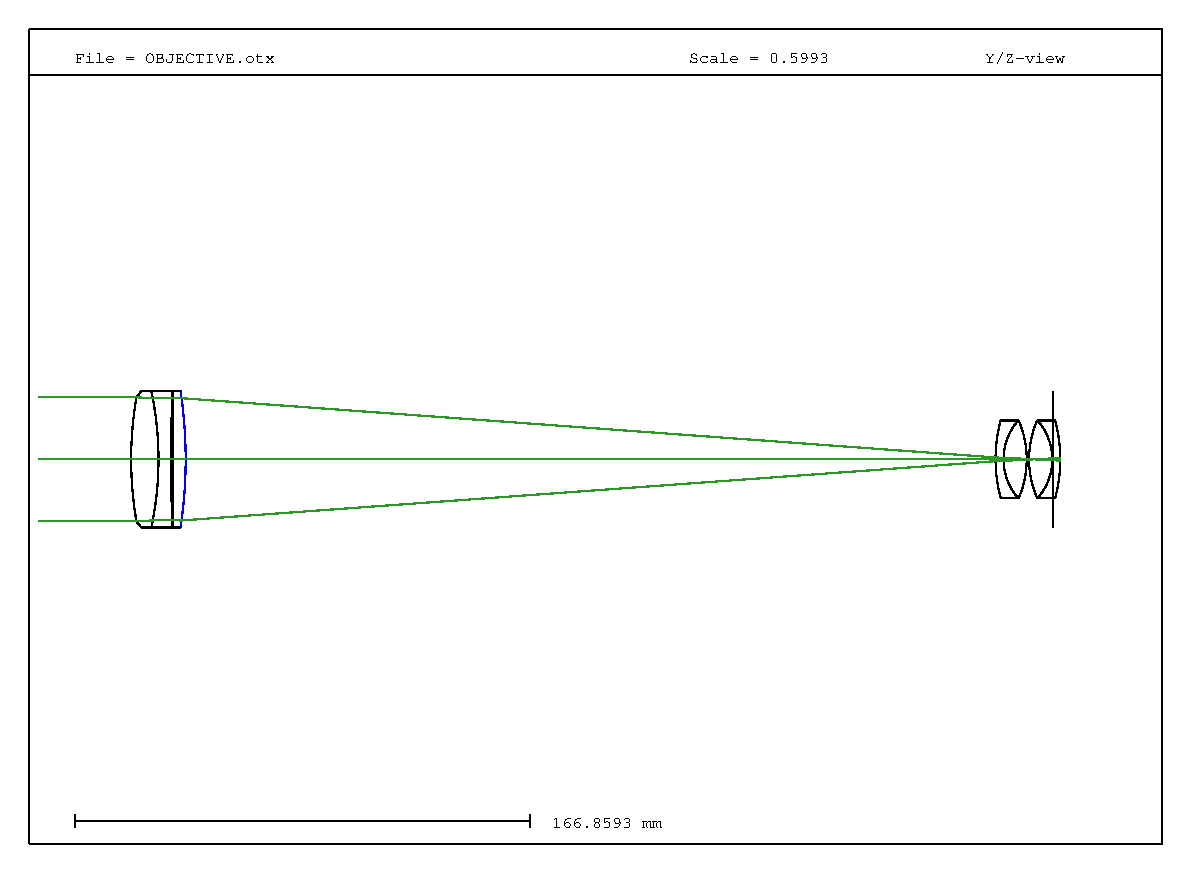
\includegraphics[width=\linewidth]{img/eps/objective_basic.eps}
    \caption{Refractor telescope design: basic schematic}%
    \label{fig:basic_refractor}
\end{figure}

\begin{figure}[htpb]
    \centering
    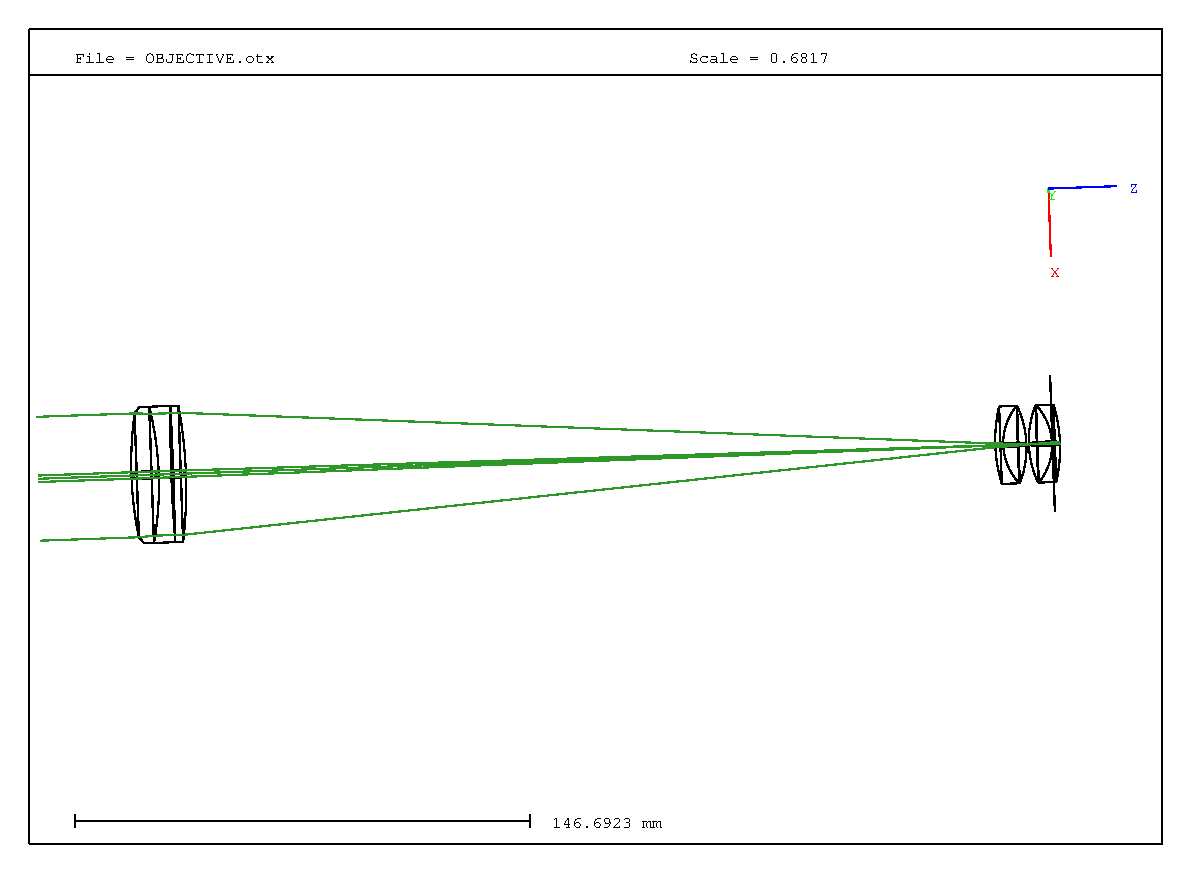
\includegraphics[width=\linewidth]{img/eps/objective.eps}
    \caption{3D schematic for the refractor telescope design.}%
    \label{fig:3d_refractor}
\end{figure}

\begin{figure}[htpb]
    \centering
    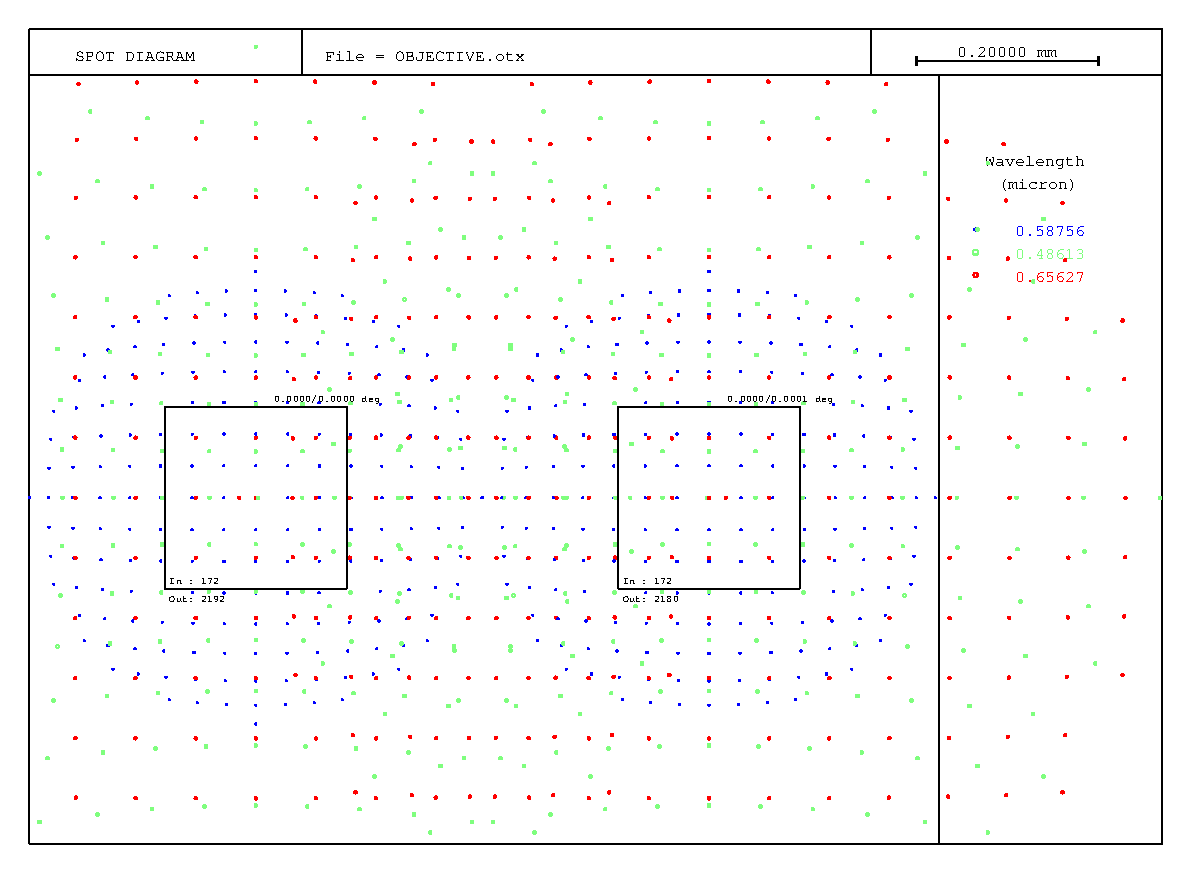
\includegraphics[width=\linewidth]{img/eps/objective_spot_diagram.eps}
    \caption{Spot diagram for the refractor telescope.}%
    \label{fig:refractor_spot_diagram}
\end{figure}

\begin{figure}[htpb]
    \centering
    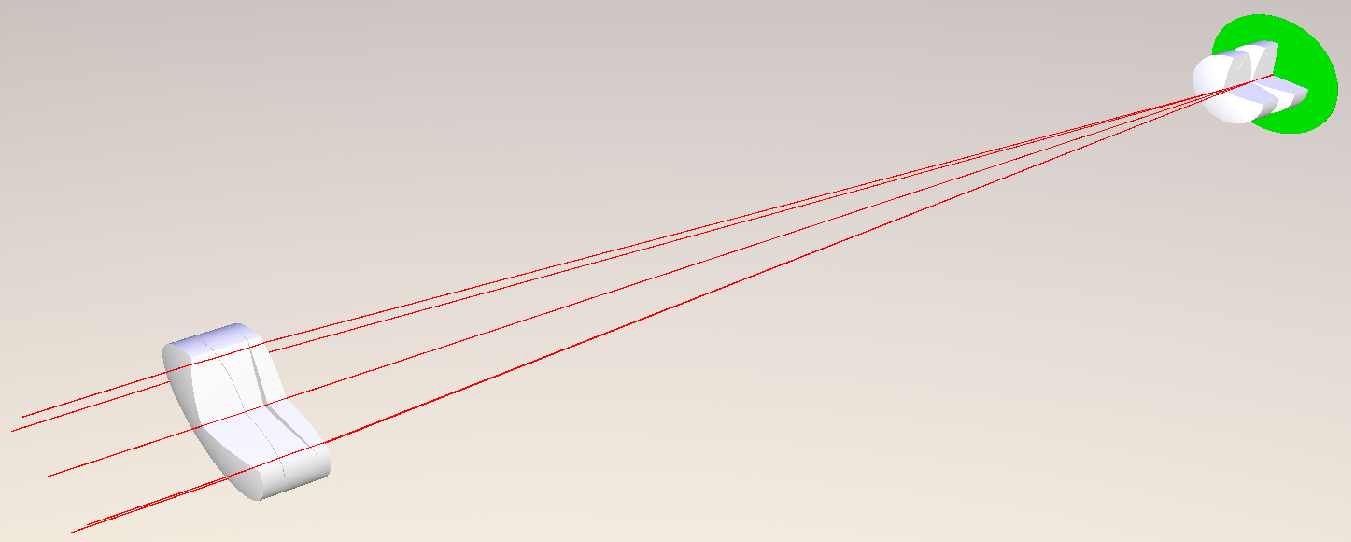
\includegraphics[width=\linewidth]{img/png/objective_render.png}
    \caption{3D rendering of the optical system}%
    \label{fig:3d_rendering_refractor}
\end{figure}

\FloatBarrier
\section*{Refractor Telescope Prescription Data}%
\label{sec:refractor_telescope_prescription_data}
\VerbatimInput{aux/objective_prescription.txt}
